
\section{KIDs specific systematics and application to CMB polarization}

In view of future utilizations of KIDs in space mission it is necessary to demonstrate the capabilities and the suitability of KIDs arrays in a space like environment. In this section we will adress some of the systematics effects that need to be taken into account during the design of futur generation detector arrays for space applications, such as the KIDs non-linearity. Here we describe the simulation method used to study the KIDs non-linearity, then we will study the KIDs linearity for different sources... \\

\subsection{Simulations}
To adress the KIDs non-linearity, we do simulations of their response to an incoming source of radiation using \rf and \cf. In this section, we give an explanation of the used method and its results.

	\subsubsection{Method}
	
The simulation method consists in modelling the response of a KID to a scan of a bright source, then to reconstruct the signal with the two methods described  in Sec.\ref{sec:signal}.

\begin{figure}[h]
\includegraphics[scale=0.54]{Figures/planets.eps}
\caption{Comparison of the incoming flux (in black) with the signals reconstructed by using method 1 (in blue) and method 2 (in red). In the top pannel and bottom pannels, the incoming fluxes are respectively $10^{3}$ and $5.10^{4}$ AU.}
\label{planet}
\end{figure}

Fig.\ref{planet} represents the reconstructed signal with different incoming flux. We observe that at a higher flux, the signal is less well reconstructed by the \rf.

In order to derive the KID non-linearity, we do a gaussian fit of the outcoming signal, to be able to plot the incoming flux as a function of the outcoming flux. This function is then fitted by a parabola :

\begin{equation}
\phi_{out} = \alpha \phi_{in} + \beta \phi_{in}^{2} ,
\label{eq:fit-nl-1}
\end{equation}

\begin{equation}
\phi_{out} = \alpha (\phi_{in} + \frac{\beta}{\alpha}  \phi_{in}^{2}).
\label{eq:fit-nl-2}
\end{equation}

The coefficient $\alpha$ is not fixed, but will be absorbed by the calibration. Eq \ref{eq:fit-nl-2} becomes :

\begin{equation}
\phi_{out} = \phi_{in} + \varepsilon \phi_{in}^{2},
\label{eq:fit-nl-3}
\end{equation}

with $\varepsilon = \frac{\beta}{\alpha}$ the non-linearity coefficient. \\
In the following paragraph, we will use the model described by Eq \ref{eq:fit-nl-3} to study the KID non-linearity when it is exposed to different sources such as : a planet, the CMB dipole, and a half wave plate (HWP).

\subsubsection{KIDs non-linearity}

The KIDs linearity has been demonstrated, over a large power range, in laboratory under realistic conditions as shown in Fig. \ref{KID-lin}. As we can see, at 300K the response of the KID is still under a linear regime.

\begin{figure}[h]
\center
	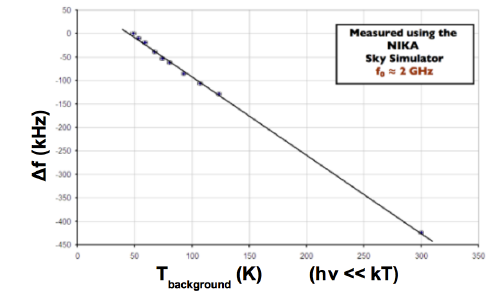
\includegraphics[scale=0.55]{Figures/KID-linearity-Monfardini2014.png}
	\caption{KID linarity demonstrated in laboratory under realistic conditions. Y-axis : frequency shift of the resonance (KID measured signal), X-axis : optical background temperature. The solid line represents the linear fit of the experimental points. Credits : \citet{2014JLTP..176..787M}.}
	\label{KID-lin}
\end{figure}

In the next paragraphs we do several simulations following the method described earlier. In these simulations we do a scanning strategy that ensures that the scanning speed is such that the number of points per beam is between 2 and 5 so that we respect Nyquist.

\paragraph{Planet only \\}

Here we simulate the scan of a planet by a KID to see if the input signal is linearly reconstruted.

\begin{figure}[h]
\center
	\includegraphics[scale=0.5]{Figures/nl-planet.eps}
	\caption{Output flux as a function of Input flux in Jy. The input signal corresponds to a planet. Blue : \rf reconstruction method, Red : \cf reconstruction method. $\varepsilon$  represented are the non-linearity cofficients for an incoming flux of 800 Jy.}
	\label{fig:nl-planet}
\end{figure}

\begin{figure}[h]
\center
	\includegraphics[scale=0.2]{Figures/diff_rf_planet.eps}
	\includegraphics[scale=0.2]{Figures/epsilon_rf_planet.eps}
	\caption{The input signal corresponds to a planet. Top : Difference between the output and input signals as a function of the input flux (Jy) and the number of points per beam. Bottom : $ln(\varepsilon)$ as a as a function of the input flux (Jy) and the number of points per beam. \cf was used to reconstruct the signal.}
	\label{fig:epsilon-rf-planet}
\end{figure}


\begin{figure}[h]
\center
	\includegraphics[scale=0.2]{Figures/diff_cf_planet.eps}
	\includegraphics[scale=0.2]{Figures/epsilon_cf_planet.eps}
	\caption{The input signal corresponds to a planet. Top : Difference between the output and input signals as a function of the input flux (Jy) and the number of points per beam. Bottom : $ln(\varepsilon)$ as a function of the input flux (Jy) and the number of points per beam. \cf was used to reconstruct the signal.}
	\label{fig:epsilon-cf-planet}
\end{figure}

Fig.\ref{nl-planet} shows the output signal, reconstructed by \rf and \cf, as a function of the input signal at different fluxes. The signal is linearly reconstructed with \rf and \cf, but becomes non-linear at higher fluxes, especially for \rf. Fig \ref{fig:epsilon-rf-planet} and \ref{fig:epsilon-cf-planet} shows that for \rf and \cf the difference between the input signal and the output signal is low ... (Cf mieux reconstruit a haut flux ??)\\

In the next parts we will see how this non-linearity progresses if we add other sources to the planet such as the CMB dipole and/or a HWP.

\paragraph{Planet and the CMB dipole \\}

The CMB dipole is a smooth gradient in the CMB temperature accross the sky. It is the result of the motion of the local group of galaxies with respect to the reference framed defined by the CMB. The CMB dipole amplitude is $\Delta T = 3.365 \pm 0.027$ mK and directed toward $(l,b) = (264.4 \degree \pm 0.3 \degree , 48.4 \degree \pm 0.5 \degree)$ in galactic coordinates \citep{2015IJMPD..2430004B}. Here we do a simulation with two incoming fluxes : a planet and the CMB dipole. 

\begin{figure}[h]
\center
	\includegraphics[scale=0.5]{Figures/nl-planet-dipole.eps}
	\caption{Output flux as a function of Input flux in Jy. The input signal corresponds to a planet and the dipole. Blue :\rf reconstruction method, Red : \cf reconstruction method. $\varepsilon$  represented are the non-linearity cofficients for an incoming flux of 800 Jy.}
	\label{fig:nl-planet-dipole}
\end{figure}

\begin{figure}[h]
\center
	\includegraphics[scale=0.2]{Figures/diff_rf_planet_dipole.eps}
	\includegraphics[scale=0.2]{Figures/epsilon_rf_planet_dipole.eps}
	\caption{The input signal corresponds to a planet and the dipole. Top : Difference between the output and input signals as a function of the input flux (Jy) and the number of points per beam. Bottom : $ln(\varepsilon)$ as a as a function of the input flux (Jy) and the number of points per beam. \rf was used to reconstruct the signal.}
	\label{fig:epsilon-rf-planet-dipole}
\end{figure}

\begin{figure}[h]
\center
	\includegraphics[scale=0.2]{Figures/diff_cf_planet_dipole.eps}
	\includegraphics[scale=0.2]{Figures/epsilon_cf_planet_dipole.eps}
	\caption{The input signal corresponds to a planet and the dipole. Top : Difference between the output and input signals as a function of the input flux (Jy) and the number of points per beam. Bottom : $ln(\varepsilon)$ as a as a function of the input flux (Jy) and the number of points per beam. \cf was used to reconstruct the signal.}
	\label{fig:epsilon-cf-planet-dipole}
\end{figure}

Fig \ref{fig:epsilon-rf-planet-dipole} and \ref{fig:epsilon-cf-planet-dipole} shows that the difference between the input signal and the output signal, and \eps, are of the same order as the ones in the simulation with only a planet, so adding the CMB dipole to the simulations does not bias the signal linearity. 

\paragraph{Planet and HWP \\} 

Many experiments, such as MAXIPOL \citep{2007ApJ...665...42J}, EBEX \citep{2010SPIE.7741E..1CR}, POLARBEAR \citep{2017JCAP...05..008T}, \nika2 \citep{2017A&A...599A..34R}, use half-wave plates (HWPs) to improve the sensitivity in polarization measurements by reducing instrumental systematics errors and low-frequency noise. Plus, it allows independant measurements of the three Stokes parameters : I, Q, and U. However, by implementing a HWP, we need to address several issues such as intensity to polarisation leakage and additional parasitic signal peaked at harmonics of the HWP rotation frequency brought by imperfections of the HWP.\\
In this simulation, we will see if adding a HWP template brings further non-linearity to the signal reconstruction. 

\begin{figure}[h]
\center
	\includegraphics[scale=0.5]{Figures/nl-planet-hwp.eps}
	\caption{Output flux as a function of Input flux in Jy. The input signal corresponds to a planet and a HWP. Blue :\rf reconstruction method, Red : \cf reconstruction method. $\varepsilon$  represented are the non-linearity cofficients for an incoming flux of 800 Jy.}
	\label{fig:nl-planet-hwp}
\end{figure}

\begin{figure}[h]
\center
	\includegraphics[scale=0.2]{Figures/diff_rf_planet_hwp.eps}
	\includegraphics[scale=0.2]{Figures/epsilon_rf_planet_hwp.eps}
	\caption{The input signal corresponds to a planet and a HWP. Top : Difference between the output and input signals as a function of the input flux (Jy) and the number of points per beam. Bottom : $ln(\varepsilon)$ as a as a function of the input flux (Jy) and the number of points per beam. \rf was used to reconstruct the signal.}
	\label{fig:epsilon-rf-planet-hwp}
\end{figure}

\begin{figure}[h]
\center
	\includegraphics[scale=0.2]{Figures/diff_cf_planet_hwp.eps}
	\includegraphics[scale=0.2]{Figures/epsilon_cf_planet_hwp.eps}
	\caption{The input signal corresponds to a planet and a HWP. Top : Difference between the output and input signals as a function of the input flux (Jy) and the number of points per beam. Bottom : $ln(\varepsilon)$ as a as a function of the input flux (Jy) and the number of points per beam. \cf was used to reconstruct the signal.}
	\label{fig:epsilon-cf-planet-hwp}
\end{figure}

As for the simulations with the planet and the planet plus dipole, we can see in Fig \ref{fig:nl-planet-hwp}, that at high fluxes the model becomes non-linear. We note that, compared to the simulation with only the planet, the non-linearity brought by the HWP is negligeable.

\paragraph{Planet, HWP and CMB dipole \\}

In this paragraph we do the same simulation but this time the incoming signals consist of : a planet, HWP template and the CMB dipole.

\begin{figure}[h]
\center
	\includegraphics[scale=0.5]{Figures/nl-planet-hwp-dipole.eps}
	\caption{Output flux as a function of Input flux in Jy. The input signal corresponds to a planet, the dipole and a HWP. Blue :\rf reconstruction method, Red : \cf reconstruction method. $\varepsilon$  represented are the non-linearity cofficients for an incoming flux of 800 Jy.}
	\label{fig:nl-planet-hwp-dipole}
\end{figure}

\begin{figure}[h]
\center
	\includegraphics[scale=0.2]{Figures/diff_rf_planet_hwp_dipole.eps}
	\includegraphics[scale=0.2]{Figures/epsilon_rf_planet_hwp_dipole.eps}
	\caption{The input signal corresponds to a planet, the dipole and a HWP. Top : Difference between the output and input signals as a function of the input flux (Jy) and the number of points per beam. Bottom : $ln(\varepsilon)$ as a as a function of the input flux (Jy) and the number of points per beam. \rf was used to reconstruct the signal.}
	\label{fig:epsilon-rf-planet-hwp-dipole}
\end{figure}

\begin{figure}[h]
\center
	\includegraphics[scale=0.2]{Figures/diff_cf_planet_hwp_dipole.eps}
	\includegraphics[scale=0.2]{Figures/epsilon_cf_planet_hwp_dipole.eps}
	\caption{The input signal corresponds to a planet, the dipole and a HWP. Top : Difference between the output and input signals as a function of the input flux (Jy) and the number of points per beam. Bottom : $ln(\varepsilon)$ as a as a function of the input flux (Jy) and the number of points per beam. \cf was used to reconstruct the signal.}
	\label{fig:epsilon-cf-planet-hwp-dipole}
\end{figure}

Like in the three precedent simulations we can see in Fig \ref{fig:nl-planet-hwp-dipole} that the signal is well reconstructed but that non-linearities appear at higher fluxes. This is especially true when we use the \rf method to reconstruct the signal. As we can see in Fig \ref{fig:epsilon-rf-planet-hwp-dipole} and Fig \ref{fig:epsilon-cf-planet-hwp-dipole}, the difference between the output and input signal, and \eps, are of the same order as the ones for the simulation with only a planet. So adding a HWP template and the CMB dipole to our simulations does not bias the linearity of the signal reconstruction.\\

(To be able to reconstruct the signal well, we need to put constraints on the scanning speed and so the number of points per beam. In order to do that, we study realistic simulations in the following paragraph, by simulating a scanning strategy typical of a satellite.) 



\subsubsection{Scanning strategy : EPIC, PLANCK}
A key factor in the design of space experiments is the scanning strategy of the instrument, as it will play a role in the systematics effect that comes from the instrument. Here, we present different simulations of scanning strategies such as the ones used in EPIC \citep{2009arXiv0906.1188B}, and PLANCK \citep{2005A&A...430..363D}.

\paragraph{EPIC \\}
For EPIC's scanning strategy, the optical axis of the telescope is inclined by 55 $\degree$ with respect to the spin axis The spin axis is inclined by 45 $\degree$ from the precession axis and it precesses around the Sun-Earth axis every hour.

\begin{figure}[h]
\center
	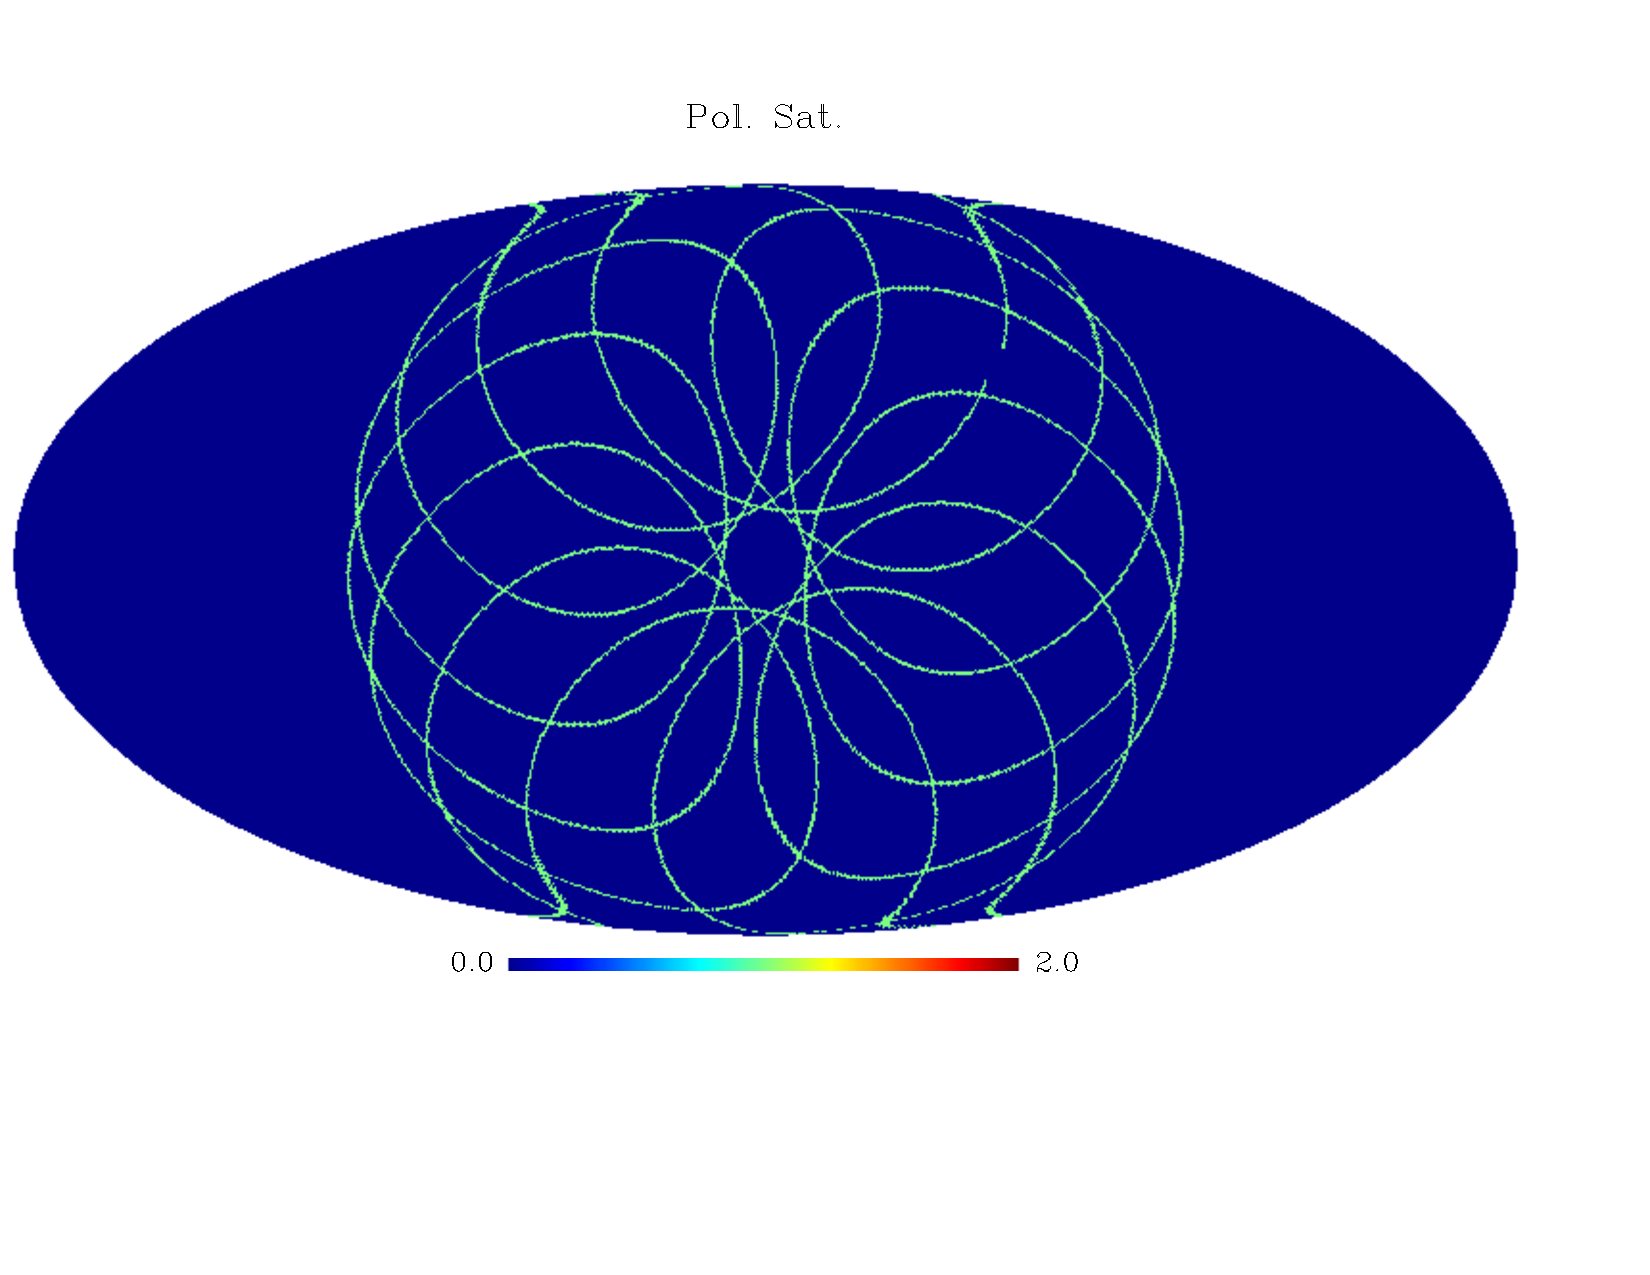
\includegraphics[scale=0.3]{Figures/scan_strat_epic.pdf}
	\caption{Simulation of EPIC's scanning strategy}
	\label{fig:strat_epic}
\end{figure}

\paragraph{PLANCK \\}
PLANCK scans large circles on the sky with a 85 $\degree$ angle between the optical axis and the spin axis. The precession angle is 7 $\degree$.

\begin{figure}[h]
\center
	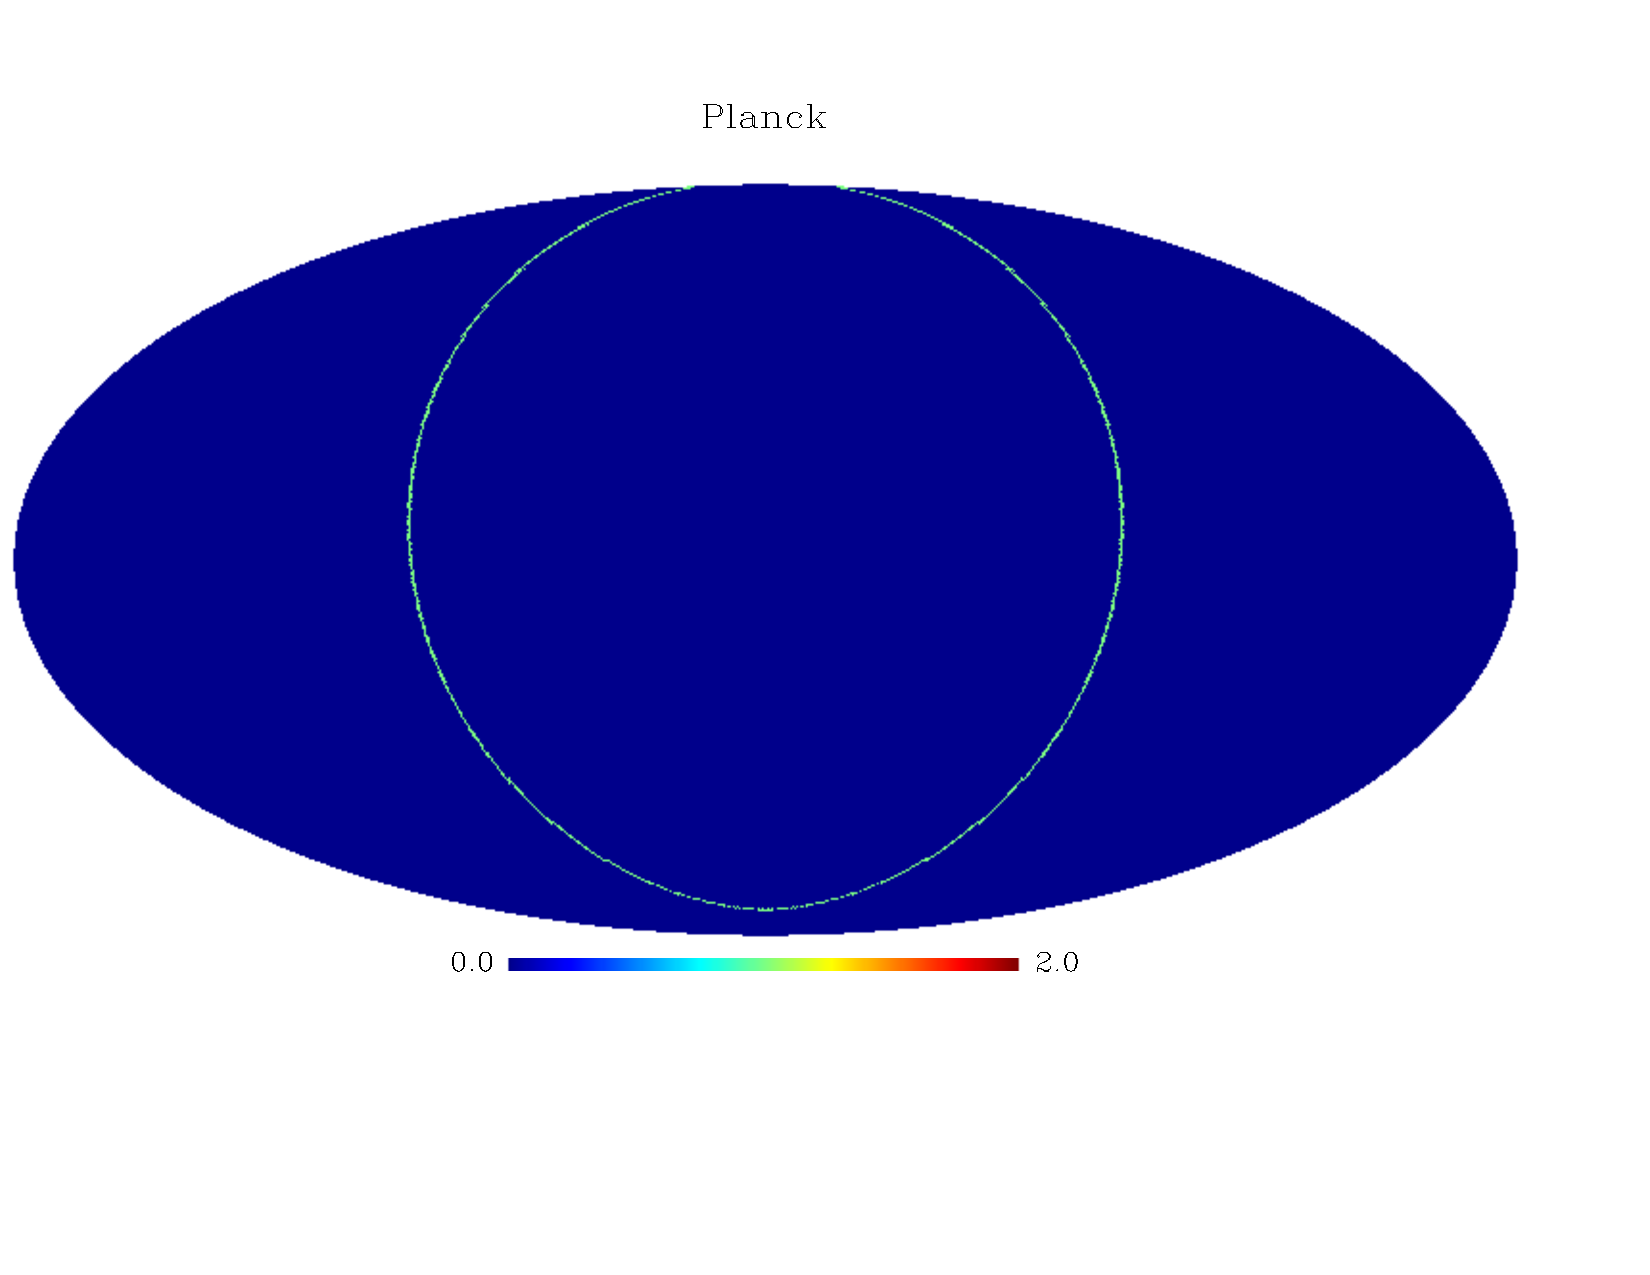
\includegraphics[scale=0.3]{Figures/scan_strat_planck.pdf}
	\caption{Simulation of PLANCK's scanning strategy}
	\label{fig:strat_epic}
\end{figure}

In the next section we will do a more realistic simulation by scanning the Galaxy and the cosmological dipole with a HWP, and by using these pointing strategies. 

\subsubsection{Results}
Pas convaincu...

%\begin{figure}[h]
%\center
%	\includegraphics[scale=0.5]{Figures/nl-planet-dipole.eps}
%	\caption{Output flux as a function of Input flux in Jy. The input signal corresponds to a planet plus a dipole. Blue : Rf reconstruction method, Red : Cf reconstruction method. Solid lines correspond to an input signal going from 0 to 5 Jy. Cross correspond to an input signal going from 0 to 0.5 Jy.}
%	\label{nl-planet-dipole}
%\end{figure}


%\begin{figure}[h]
%	\includegraphics[scale=0.53]{Figures/epsilon.eps}
%	\caption{KID non-linearity coefficient $\varepsilon$ as a function of number of points per $FWHM$. $\varepsilon$ was determined by using method 1 and method 2, for incoming fluxes between $1.10^{2}$ and $5.10^{4}$ AU.}
%	\label{results_epsilon}
%\end{figure}

%Fig.\ref{results_epsilon} shows the non-linearity coefficient $\varepsilon$ derived, with the model described by Eq.\ref{fit_NL}, for different incoming flux. We can see that the non-linearity coefficients found by method 2 are lower than those found by method 1. Plus, the first method has shown that it is limited for incoming flux higher than $10^{4}$ as the signal is not perfectly reconstructed, whereas limite de la method 2.... To conclude, the second method is better than the first one which already reconstructed the signal very well.\\
%
%Now that we have derived the non-linearity coefficient $\varepsilon$, we will see how to 


\subsection{Application to CMB maps and power spectra estimations}
The measurement of CMB polarization, and especially the detection of B modes, is one of the major challenges in modern cosmology. In this paper, we show that the KIDs systematic effect such as the non-linearity does not affect them from detecting B modes.

In this section we look at the next order correction, meaning that we will focus on the non-linear term produced by the detector and the way that we reconstruct the signal. A measure done by the KID is defined by $m = T + P$, with $T$ and $P$ representing the temperature and polarization. The non-linearity is characterized  by the $\varepsilon$ coefficient in $ m = m_{1} + \varepsilon m_{1}^{2}$. We have : 

\begin{equation}
\begin{split}
m & = m_{1} +\varepsilon' (T+P)^{2} \\
 & = T + P + \varepsilon'(T^{2} + P^{2} + 2TP) 
\end{split}
\end{equation}

Therefore, knowing that $T=I$ and $P = Q\cos(2\alpha) + U \sin(2\alpha)$, the polarized equation with a non-linear term is given Eq. \ref{eq-NL}.

\begin{equation}
m  \simeq (I + \varepsilon' I^{2}) + (Q + 2\varepsilon' IQ) \cos(2\alpha) + (U + 2 \varepsilon' IU) \sin(2\alpha)
\label{eq-NL}
\end{equation}

The non-linear coefficient $\varepsilon'$ is induced by the detector and the method used to reconstruct the signal.

The non-linearity coefficient $\varepsilon'$ does not intervene in the pointing strategy, in fact it is a systematic effect of the instrument and as a consequence will always impact our measurments. \\
To take into account this effect we simulate CMB maps with a PLANCK pointing strategy (citer ref) which follows Eq. \ref{eq-NL}. We used the HEALPix package/Ring pixelization scg=heme of the sphere (REF) to create simulated maps and to estimate power spectra.

%For allmaps we use the HEALPix Ring pixelization scheme of the sphere (Gorski et al. 1999)
%The input CMB power spectra were created with CAMB (Lewis & Challinor 2011) and we used the HEALPix package (Gorski et al. 2005) to create simulated maps, and to estimate power spectra

Eq. \ref{eq-NL} is translated in the the power spectrum by Eq. \ref{eq-Cl}.

\begin{equation}
C_{l}^{s} \propto p^{2} \varepsilon^{2} C_{l},
\label{eq-Cl}
\end{equation}
Where $C_{l}^{s}$ is the systematic power spectra.\\

We generate I, Q, U maps from observed $C_{l}$ to which we apply the non-linear mapping described by Eq.\ref{eq-NL}. This will produce spurious polarization signals from which we can derive modified $C_{l}^{s}$ and $\varepsilon$ represented in Eq. \ref{eq-Cl}. We found :

\begin{equation}
\varepsilon^{2} \simeq 4.10^{-7}.
\label{epsilon}
\end{equation}

\begin{figure}[h]
\center
	\includegraphics[scale=0.55]{Figures/cl.eps}
	\caption{cl}
	\label{fig:cl}
\end{figure}

This non-linearity can lead to leakage of the CMB temperature signal into the polarization maps and consequently can induce spurious polarization signals which could prevent us from detecting B mode polarization. The leakage effect is represented by the coefficient $\varepsilon$ of Eq. \ref{eq-Cl}. As a result, to be able to detect B mode polarization, the non-linearity coefficient related to the signal reconstruction must be lower than $\varepsilon^{2} \simeq 4.10^{-7}$.

%To do so, we calculate the non-linearity coefficient $\varepsilon'$ given by Eq.\ref{eq-NL} with a tolerance on mode B contamination by generating I, Q, U maps from observed $C_{l}$. Then we apply the non linear mapping described by Eq.\ref{eq-NL}, this will generate spurious signal from which we derive modified $C_{l}$. 

\subsection{Cosmic rays impact on KIDs array}

One of the major problems for space based missions is the impact of an intense flux of high energy particles, referred to as Cosmic Rays (CR) on the detectors. Primary CR are produced by the Sun and by other galactic sources. They are mostly composed by protons (90\%), helium nuclei (9\%) and a few heavier nuclei and electrons (1\%). The CR spectrum is peaked aroud 200 MeV, thus the particles have sufficient energy to penetrate the detectors and give an unwanted signal. The Planck satellite \citep{2014A&A...571A..10P} has demonstrated that the impact of CR on the detectors are a key problem for space missions. Indeed, the glitches caused by CR can mask the real data and induce a loss of an important fraction of it.\\
Experiments have been done to construct a setup that allows to study the behavior of KIDs arrays under typical conditions of a space-borne observatory, and establish the compatibility of KIDs with a space environment \citep{2016A&A...592A..26C,2016SPIE.9914E..0NM}. When the detector is hit by a CR there is a lapse of time during which the sensor is 'blind' to the incoming scientific data. The length of this dead-time depends on the response time of the KID (time constant) which is determined by the quasi particle lifetime. \citet{2012ApPhL.100w2601M} have shown for KID, this time constant is equal to about tens of microseconds which is faster than bolometers (from 5-10 ms to 2s). This means that for the same CR hit, less data is lost when using KIDs arrays. Plus, the experiments have confirmed the fact that KID recover their initial state in less than 5 milliseconds. Finally, \citet{2016SPIE.9914E..0NM} concluded that the percent level of data loss per pixel by a KIDs array placed in a space environment is about 1 \% compared to 15 \% for Planck HFI bolometers.\\ The KID technology shows promising results for compatibility with a space-borne mission, as their extremely short glitch time constant permits to greatly reduce the data loss fraction due to CR impacts. 

